\chapter{Syntetický gradient neurónových sieti}

\label{synth_grad} % id kapitoly pre prikaz ref

Trénovanie neurónovej siete pozostáva z dvoch fáz. Fázy dopredného šírenia a fázy spätného šírenia chyby. Vo fáze dopredného šírenia je vstupný signál šírený orientovanými hranami medzi jednotlivými vrstvami neurónovej siete. Každá vrstva neurónovej siete je považovaná za výpočtový krok ktorý transformuje vstupné dáta (signály) \cite{Jaderberg2016}. Po ukončení fázy dopredného šírenia je výstupom neurónovej siete predikovaná hodnota. Na základe predikovanej hodnoty je možné definovať chybu neurónovej siete (tiež známa ako \textit{chyba predikcie}). Akonáhle je dostupná hodnota chyby neurónovej siete, aktivuje sa druhá fáza, fáza spätného šírenia chyby. Hodnota chyby je spätne šírená celou neurónovou sieťou. Táto chyba umožňuje generovať gradient, ktorý je nevyhnutný pre úpravu váh jednotlivých vrstiev neurónovej siete \cite{Jaderberg2016}. Hodnota chyba neurónovej siete je výsledkom chybovej funkciou $L(\hat{y}, y)$, kde $\hat{y}$ je predikovaná hodnota a $y$ je skutočná hodnota (ďalej len ako supervízia). Hodnota gradientu je generovaná samostatne v každej vrstve, na základe obdržanej chyby. Vrstva ktorá obdrží hodnotu chyby, upraví svoje váhy a následne pošle túto hodnotu chyby ďalším vrstvám \cite{Goh1995, Czarnecki2017}. 

V oboch fázach trénovania neurónovej siete dochádza k takzvanému \textit{uzamknutiu výpočtu} vrstiev neurónovej siete. Uzamknutie výpočtu vrstiev predstavuje neefektívne pristupovanie k jednotlivým vrstvám neurónovej siete. V celom systéme trénovania neurónovej siete sa nachádza vždy len jedna aktívna vrstva. Ostatné vrstvy sú blokované, resp. čakajú na získanie všetkých potrebných informácií na to, aby mohli vykonať vlastné operácie (či už transformáciu dát alebo úpravu váh). Typy uzamknutí výpočtu delíme na \cite{Jaderberg2016}:
\begin{enumerate}
\item  \textit{Uzamknutie v smere dopredného šírenia} - vrstva $i$ nemôže vykonať transformáciu dát, pokiaľ vrstva $i-1$ nepošle transformované dáta.
\item  \textit{Uzamknutie úpravy váh} - žiadna vrstva nemôže upraviť váhy dokiaľ všetky vrstvy nedokončia fázu dopredného šírenia.
\item  \textit{Uzamknutie v smere spätného šírenia chyby} - vrstva $i$ nemôže upraviť svoje váhy, pokiaľ vrstva $i+1$ nepošle hodnotu chyby.
\end{enumerate}

Vzhľadom k tomu, že v celom systéme je vždy len jedna vrstva aktívna, tak jednotlivé vrstvy sú závislé na iných vrstvách:
\begin{itemize}
    \item vrstva $i$ je závislá na vrstve $i-1$ vo fáze dopredného šírenia.
    \item vrstva $i$ je závislá na vrstve $i+1$ vo fáze spätného šírenia chyby.
\end{itemize}
Závislosť jednotlivých vrstiev na iných vrstvách zapríčiňuje sekvenčné (synchrónne) fungovanie neurónovej siete. Synchrónny prístup spôsobuje, že všetky vrstvy ktoré nevykonávajú úpravu váh alebo transformáciu dáta sú nečinné \cite{Jaderberg2016}.

V ďalších častiach povieme viacej o tom, ako efektívne zamestnať jednotlivé vrstvy zatiaľ čo iné vrstvy vykonávajú prisluchajúce operácie. Vysvetlíme, ako paralelizovať výpočtové kroky spätného šírenia chyby a ako odstrániť uzamknutie úpravy váh a uzamknutie v smere spätného šírenia chyby.

\section{Funkcia syntetického gradientu}
\label{understanding_SG} % id kapitoly pre prikaz ref
Trénovanie neurónovej siete pozostáva zo sekvenčných krokov ktoré obmedzujú potenciál neurónovej siete. Vrstvy ktoré nevykonávajú transformáciu dát alebo úpravu váh sú nútené čakať na vrstvy, na ktorých sú závislé. Vrstva \textit{i} vo fáze dopredného šírenia je nútená čakať na vrstvu \textit{i-1} a vo fáze spätné šírenia chyby na vrstvu \textit{i+1} \cite{Jaderberg2016}. 

Vrstva $i+1$ vykonáva transformáciu dát až keď obdrží transformované dáta od vrstvy $i$. Vrstva $i$ je schopná úpravy váh akonáhle odošle transformované dáta. Tento úkon nie je možné vykonať vzhľadom na \textit{uzamknutie úpravy váh} a \textit{uzamknutie v smere spätného šírenia chyby}. Z dôvodu uzamknutia vypočtu, vrstva $i$ upravuje váhy až po získaní hodnoty chyby od vrstvy $i+1$ \cite{Jaderberg2016}.


Úprava váh je realizovaná pomocou gradientu $\partial L/\partial h_i$, kde $L$ je chybová funkcia neurónovej siete a $h_i$ je funkcia transformácie dát vrstvou $i$ (aktivačná funkcia) \cite{Goh1995}. Vyššie sme uviedli, že váhy jednotlivých vrstiev sa upravujú vo fáze spätného šírenia chyby. Algoritmus spätného šírenia chyby na úpravu váh vyžaduje hodnotu chyby predikcie z výstupu neurónovej siete. Získavanie hodnoty predikcie z výstupu neurónovej siete zapríčiňuje všetky tri typy uzamknutia výpočtu neurónovej siete \cite{Goh1995, Czarnecki2017, Jaderberg2016}.

Cieľom syntetického gradientu je umožniť jednotlivým vrstvám úpravu váh hneď po odoslaní transformovaných dát ďalšej vrstve. Syntetický gradient predstavuje aproximáciu skutočného gradientu a je generovaný modulom syntetického gradientu. Vrstva ktorá realizovala dopredné šírenie, okamžite obdrží od modulu syntetického gradientu aproximovaný skutočný gradient (syntetický gradient). Poskytnutý syntetický gradient je použitý na úpravu váh danej vrstvy. Implementácia syntetického gradientu zabezpečuje odstránenia uzamknutia úpravy váh a uzamknutia v smere spätného šírenia chyby \cite{Jaderberg2016}. 

Skutočný gradient je vo fáze spätného šírenia chyby definovaný ako \cite{Goh1995, Jaderberg2016}:
\begin{equation}
    \frac{\partial L}{\partial \theta \textsubscript{i}} = f\textsubscript{Bprop}((h\textsubscript{i},x\textsubscript{i},y\textsubscript{i},\theta\textsubscript{i}),...)\frac{\partial h\textsubscript{i}}{\partial \theta \textsubscript{i}}
\end{equation}
kde \textit{h}\textsubscript{i} sú transformované dáta, \textit{x}\textsubscript{i} sú vstupné dáta, \textit{y}\textsubscript{i} je supervízia, $\theta_i$ je váhový vektor a \textit{L} je chybová funkcia ktorú sa snažíme minimalizovať. Aproximácia skutočného gradientu predstavuje odstránenie závislostí funkcie $f_{Bprop}$ na hodnotách $x_i$, $y_i$ a $\theta_i$. Syntetický gradient $\hat{f}\textsubscript{Bprop}(h\textsubscript{i})\frac{\partial h\textsubscript{i}}{\partial \theta \textsubscript{i}} $
je závislý len na transformovaných dátach $h_i$ \cite{Jaderberg2016}.  

Generovanie syntetického gradientu nevyžaduje dodatočné informácie od iných vrstiev. Syntetický gradient $\hat{\delta}_i$ je závislý len od transformovaných dát $h_i$ a vo fáze úpravy váh nevzniká závislosť vrstvy $i$ na iných vrstvách. Použitie aproximovanej funkcie spätného šírenia chyby na generovanie syntetického gradientu zabezpečuje odstránenie uzamknutia úpravy váh a uzamknutia v smere spätného šírenia chyby \cite{Jaderberg2016}.

Syntetický gradient je generovaný modulom syntetického gradientu. Vrstva $i$ komunikuje s modulom syntetického gradientu $M_{i+1}$ prostredníctvom oddeleného neurónového rozhrania, DNI (z angl. Decoupled Neural Interface). Toto rozhranie realizuje aproximáciu funkcie spätného šírenia chyby \cite{Czarnecki2017}. Vrstva \textit{i} komunikuje s DNI akonáhle transformuje všetky dáta. Po odoslaní transformovaných dát do DNI, vrstva \textit{i} obdrží syntetický gradient ktorý jej umožní okamžitú úpravu váh (viď Obr. \ref{komunikaciaDNI}) \cite{Jaderberg2016}.

Chyba neurónovej siete je definovaná ako $L\textsubscript{i}=L(h\textsubscript{i},y\textsubscript{i})$, kde \textit{y}\textsubscript{i} sú skutočné hodnoty očakávané na výstupe vrstvy $i$ a $h_i$ sú dáta transformované vrstvou $i$. Trénovanie jednotlivých vrstiev neurónovej siete spočíva v úprave váh $\theta\textsubscript{i}$ za účelom minimalizovania hodnoty chyby $L\textsubscript{i}$, kde $i$ určuje poradie vrstvy neurónovej siete, pričom $I$ je posledná vrstva. Algoritmus spätného šírenia chyby, vykonáva úpravu váh ako \cite{Jaderberg2016, Goh1995}:
\begin{equation}
    \theta\textsubscript{i} \leftarrow \theta\textsubscript{i} - \alpha \frac{\partial L (h\textsubscript{I},y\textsubscript{I})}{\partial h \textsubscript{i}}\frac{\partial h \textsubscript{i}}{\partial \theta \textsubscript{i}} ;\qquad \frac{\partial L(h\textsubscript{I},y\textsubscript{I})}{\partial h \textsubscript{I}} = \delta\textsubscript{i}
\end{equation}
kde $\alpha$ je krok učenia, $h_I$ je hodnota na výstupe neurónovej siete, $y_I$ je očakávaná hodnota na výstupe neurónovej siete, $h_i$ je transformácia aktivačnou funkciou a $\delta_i$ predstavuje hodnotu gradientu ktorá je získaná zo spätného šírenia chyby \cite{Czarnecki2017, Goh1995, Jaderberg2016}.

 
 Modul syntetického gradientu predstavuje jednoduchú neurónovú sieť ktorá je trénovaná na predikciu skutočného gradientu. Modul syntetického gradientu $M_{i+1}$ aproximuje hodnotu skutočného gradientu na základe transformovaných dát $h_i$ ako $\hat{\delta\textsubscript{i}}=M\textsubscript{i+1}(h\textsubscript{i})$, kde syntetický gradient $\hat{\delta\textsubscript{i}} = \widehat{\partial L_i/\partial h_i}\simeq\partial L\textsubscript{i}/\partial h \textsubscript{i}$ \cite{Czarnecki2017}. Syntetický gradient nahrádza skutočný gradient a úprava váh je realizovaná výhradne pomocou syntetického gradientu ako \cite{Jaderberg2016}:
\begin{equation}
    \theta\textsubscript{i} \leftarrow \theta\textsubscript{i} - \alpha \hat{\delta\textsubscript{i}}\frac{\partial h \textsubscript{i}}{\partial \theta \textsubscript{i}}
\end{equation}
Vzhľadom k tomu, že syntetický gradient je obdržiavaný z DNI, tak úprava váh vrstvy \textit{i} môže byť realizovaná hneď ako vrstva \textit{i} pošle transformované dáta \textit{h}\textsubscript{i} do DNI. Táto metóda sa opiera o fakt, že syntetický gradient je definovaný ako $\hat{\delta_i} = \partial L_i / \partial h_i$ a teda nevyžaduje žiadne dodatočné informácie od iných vrstiev \cite{Czarnecki2017}.

Vrstva \textit{i} odosiela transformované dáta do DNI ale tiež aj vrstve $i+1$. Vzhľadom k tomu, že vrstva $i$ okamžite obdrží syntetický gradient, tak je zabezpečené paralelizovanie procesov úpravy váh (vrstvou $i$) a transformáciou dát (vrstvou $i+1$). Ako vidíme na Obrázku \ref{komunikaciaDNI}, vrstva \textit{f}\textsubscript{A} odošle transformované dáta vrstve \textit{f}\textsubscript{B} ale tiež aj do \textit{M}\textsubscript{B}. Vrstva \textit{f}\textsubscript{B} je schopná ďalej vykonávať dopredné šírenie (transformovať prijaté dáta a posielať ich ďalším vrstvám) a paralelne s ňou, vrstva \textit{f}\textsubscript{A} upravuje svoje váhy.

\begin{figure}
%vlozenie samotneho obrazku vycentrovaneho a vhodnej velkosti
%obrazok je v subore images/cervik.png
\centerline{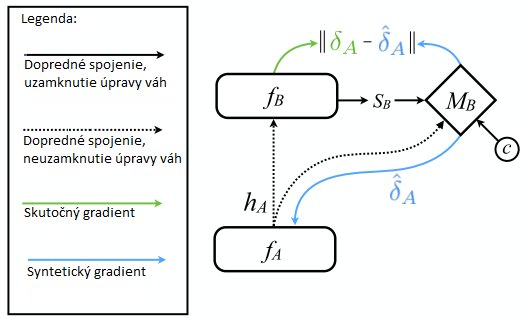
\includegraphics[width=0.4\textwidth]{images/DNI}}
%popis obrazku
\caption[Komunikácia vrstiev s DNI]{Akonáhle vrstva \textit{f}\textsubscript{A} transformuje dáta (\textit{h}\textsubscript{A}), odošle ich vrstve \textit{f}\textsubscript{B} a tiež pomocou DNI do \textit{M}\textsubscript{B}. Vrstva $f(A)$ upravuje svoje váhy paralelne s tým ako vrstva $f(B)$ transformuje prijaté dáta. $M_B$ upravuje svoje váhy pomocou hodnoty chyby $S_B$ obdržanej od $f_B$. $M_B$ môže byť podmienené nejakou podmienkou $c$ \cite{Jaderberg2016}.}
\label{komunikaciaDNI}
%id obrazku, pomocou ktoreho sa budeme na obrazok odvolavat
\end{figure}

Keďže pri využití DNI, žiadna vrstva nečaká na skutočný gradient, tak je zabezpečená paralelizácia dopredného šírenia a úpravy váh. DNI nahrádza štandardné neurónové medzivrstvové rozhranie za účelom šírenia gradientu a paralelného dopredného šírenia. Výsledkom je odstránenie \textit{uzamknutia úpravy váh} a \textit{uzamknutia v smere spätného šírenia} z procesu trénovania neurónovej siete \cite{Jaderberg2016}.

Zatiaľ nie je úplne jasné, či použitie DNI a syntetického gradientu celkovo, má negatívny vplyv na presnosť neurónovej siete. Podľa experimentov \cite{Jaderberg2016, Czarnecki2017} nie je zaznamenaný žiaden signifikantne negatívny vplyv. Táto metóda vychádza z empirického predpokladu, že aproximácia skutočného gradientu je schopná priblížiť sa skutočnému gradientu natoľko, že syntetický gradient poskytnutý modulmi syntetického gradientu bude zhodný so skutočným gradientom. 

\section{Modul syntetického gradientu a DNI}
\label{SGaDNI}

DNI je druh rozhrania slúžiaceho na komunikáciu jednotlivých vrstiev neurónovej siete s modulmi syntetického gradientu. Modul syntetického gradientu predstavuje jednoduchú doprednú neurónovú sieť s jednou skrytou vrstvou. Modul syntetického gradientu $M_{i+1}$ na vstupe očakáva transformované dáta $h_i$ poskytnuté vrstvou $i$. Obdržané dáta sú dopredne šírené modulom syntetického gradientu ktorého výstupom je predikovaný (syntetický) gradient. Predikovaný gradient je spätne šírený vrstve $i$. Keďže generovanie syntetického gradientu nevyžaduje žiadne dodatočné informácie z iných vrstiev, tak vrstva $i$ \cite{Jaderberg2016}:
\begin{itemize}
\item je schopná upraviť svoje váhy aj napriek tomu, že vrstvy $i-1$ a $i+1$ ešte neukončili fázu dopredného šírenia
\item je schopná upraviť svoje váhy aj napriek tomu, že vrstva $i+1$ ešte neukončila úpravu svojich váh
\end{itemize}

Kapitola \ref{understanding_SG} uvádza, že modul syntetického gradientu sa usiluje o čo najpresnejšiu aproximáciu skutočného gradientu. Kvalita predikcie gradientu je zvyšovaná trénovaním modulu syntetického gradientu. Trénovanie modulu syntetického gradientu predstavuje úpravu váh $\phi_i$ za účelom minimalizácie chyby predikcie modulu syntetického gradientu \cite{Jaderberg2016}. Modul syntetického gradientu je trénovaný v rovnakom čase ako je trénovaná neurónová sieť samotná.  Paralelne s úpravou váh jednotlivých vrstiev neurónovej siete sú upravované aj váhy modulu syntetického gradientu \cite{Czarnecki2017}.

Algoritmus syntetického gradientu, ktorý je využitý na trénovanie neurónovej siete pozostáva z niekoľkých krokov \cite{Jaderberg2016, Czarnecki2017}:

\begin{enumerate}
    \item Vrstva $f_i$ odošle transformované dáta $h_i$ vrstve $f_{i+1}$ a modulu syntetického gradientu $M_{i+1}$.
    \item Modul syntetického gradientu $M_{i+1}$ generuje syntetický gradiedient $\hat{\delta}_i=M_{i+1}(h_i)$.
    \item Syntetický gradient $\hat{\delta}_i$ je spätne šírený vrstve $f_i$, ktorá okamžite upraví svoje váhy $\theta_i$.
    \item Vrstva $f_{i+1}$ vykoná transformáciu obdržaných dát, ktoré dopredne šíri ďalším vrstvám. Akonáhle vrstva $f_{i+1}$ obdrží gradient (bez ohľadu na to, či syntetický alebo skutočný), upraví svoje váhy $\theta_{i+1}$ a tento gradient posiela modulu syntetického gradientu $M_{i+1}$.
    \item Modul syntetického gradientu $M_{i+1}$ obdržaný gradient $\delta_i$ považuje za supervíziu (očakávanú hodnotu). Modul syntetického gradientu $M_{i+1}$ si na základe obdržaného gradientu $\delta_i$ upraví váhy $\phi_{i+1}$ tak, aby čo najviac minimalizoval $L^2$ vzdialenosť medzi predikovaným gradientom $\hat{\delta}_i$ a skutočným gradientom $\delta_i$, ${\left\Vert \hat{\delta}\textsubscript{i} - \delta\textsubscript{i}\right\Vert}_{2}^2$.
\end{enumerate}

Syntetický gradient je možné použiť na oddelenie všetkých vrstiev neurónovej siete. Každá vrstva, s výnimkou vstupnej a výstupnej vrstvy, môže mať pripojený vlastný modul syntetického gradientu. Pre výstupnú vrstvu nie je potrebné mať modul syntetického gradientu vzhľadom k tomu, že výstupnej vrstve je okamžite poskytnutý skutočný gradient \cite{Jaderberg2016}.

Vrstvy, ktorým je zabezpečená komunikácia s modulom syntetického gradientu, na úpravu svojich váh využívajú výhradne syntetický gradient poskytnutý pripojeným modulom (viď Obrázok \ref{multiDNI} c)). Pri štandardnom spätnom šírení chyby, vrstva $f_{i+1}$ šíri obdržaný gradient vrstve $f_i$ (viď Obrázok \ref{multiDNI} a)). Pri implementácii modulu syntetického gradientu, vrstva $f_{i+1}$ šíri obdržaný gradient modulu syntetického gradientu $M_{i+1}$. Modul syntetického gradientu $M_{i+1}$ obdržaný gradient považuje za skutočný aj napriek tomu, že ide len o aproximovanú verziu skutočného gradientu \cite{Jaderberg2016}.

\begin{figure}
%vlozenie samotneho obrazku vycentrovaneho a vhodnej velkosti
%obrazok je v subore images/cervik.png
\centerline{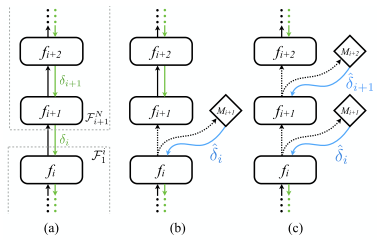
\includegraphics[width=0.6\textwidth]{images/multiDNI}}
%popis obrazku
\caption[Porovnanie architektúr neurónových sieti s implementáciou DNI]{a) Štandardná neurónová sieť ktorej vrstvy upravujú svoje váhy podľa skutočného gradientu získaného spätným šírením chyby \cite{Goh1995}. b) Neurónová sieť s jedným modulom syntetického gradientu. Vrstva $f_i$ obdržiava syntetický gradient $\hat{\delta}\textsubscript{i}$ od modulu syntetického gradientu $M_{i+1}$. Vrstva $f_{i+2}$ disponuje skutočným gradientom ktorý spätne šíri vrstve $f_{i+1}$ a tá ho následne poskytne modulu syntetického gradientu $M_{i+1}$. c) Vrstva $f_{i+1}$ obdržiava syntetický gradient $\hat{\delta}_{i+1}$ od modulu syntetického gradientu $M_{i+2}$. Tento gradient je spätne šírený modulu syntetického gradientu $M_{i+1}$. \cite{Jaderberg2016}}
\label{multiDNI}
%id obrazku, pomocou ktoreho sa budeme na obrazok odvolavat
\end{figure}

Na obrázku \ref{komunikaciaDNI} si môžeme všimnúť uzol \textit{c} spojený s modulom syntetického gradientu \textit{M}\textsubscript{B}. Uzol \textit{c} poskytuje dodatočnú informáciu pre daný modul syntetického gradientu. Môže ísť o nejaký druh kontextu v ktorom sa neurónová sieť nachádza, alebo najčastejšie o informáciu aká hodnota je očakávaná na výstupe neurónovej siete (supervízia). Akonáhle je táto informácia dostupná, tak modul syntetického gradientu \textit{M}\textsubscript{i+1} produkuje syntetický gradient $\hat{\delta}\textsubscript{i} = M\textsubscript{i+1}(h\textsubscript{i},c)$.

\section{Kombinácia spätne-šíreného a syntetického gradientu}

Algoritmus $BP(\lambda)$ umožňuje trénovanie neurónovej siete kombináciou spätne-šíreného gradientu a syntetického gradientu, stochastickým spôsobom. Parameter $\lambda$ určuje, ktorý z dvoch dostupných gradientov bude použitý na úpravu váh. Algoritmus umožňuje využívať spätne šírený gradient až dovtedy, dokiaľ je dostupný a dôveryhodný. V prípade ak vybraný gradient nie je dostupný, tak existuje alternatíva (modul syntetického gradientu), ktorá poskytne nový gradient \cite{Jaderberg2016}.
\begin{comment}
Syntetický gradientu $\hat{\delta}_i\approx\partial L/\partial h\textsubscript{i}$, predstavuje aproximovanú verziu skutočného gradientu $\partial L/\partial h\textsubscript{i}$. Syntetický gradient $\hat{\delta}_i$ je výsledkom funkcie $\hat{\delta}_i=SG(h_i, \phi_{i+1})$, kde $h_i$ sú transformované dáta a $\phi_{i+1}$ je váhový vektor modulu syntetického gradientu $M_{i+1}$. S využitím syntetického gradientu je minimalizovaná chyba neurónovej siete
\begin{equation}
    \frac{\partial L}{\partial\theta\textsubscript{i}}=\frac{\partial L}{\partial h\textsubscript{i}}\frac{\partial h\textsubscript{i}}{\partial\theta\textsubscript{i}} \approx \hat{\delta}\textsubscript{i}\frac{\partial h\textsubscript{i}}{\partial\theta\textsubscript{i}},
\end{equation}
kde $\theta_i$ je váhový vektor vrstvy $i$ a $L$ je chyba predikcie neurónovej siete  \cite{Jaderberg2016}. 

Pre docielenie čo najpresnejšej predikcie gradientu je trénovaný aj modul syntetického gradientu. Modul syntetického gradientu $M_{i}$ za supervíziu považuje gradient poskytnutý vrstvou $i$, $\delta_i = \hat{\delta}_{i+1} \frac{\partial h_{i+1}}{\partial h_i}$. Po obdržaní supervízie $\delta_i$ nastáva úprava váh modulu syntetického gradientu $\phi_i$, ktorá minimalizuje kvadratickú chybu $L_{M_i}=(\delta_i - \hat{\delta}_i)^2$ ako $\partial L_{M_i}/\partial \phi_i$ \cite{Jaderberg2016}.
\end{comment}

Parameter $\lambda$ je množina stochasticky vygenerovaných binárnych hodnôt, kde $\lambda\textsubscript{i}\in\{0, 1\}$ a \textit{i} je poradie vrstvy v rámci neurónovej siete \cite{Jaderberg2016}. Každá vrstva neurónovej siete na úpravu svojich váh používa (viď Obrázok \ref{BPlambdaAlgoritmus}):
\begin{itemize}
    \item gradient šírený spätnou propagáciou chyby s pravdepodobnosťou $P=\lambda$
    \item syntetický gradient obdržaný z modulu syntetického gradientu s pravdepodobnosťou $P=(1-\lambda)$.
\end{itemize}
Gradient $g_i$ ktorý obdrží vrstva $i$ je parametrizovaný súčet gradientu šíreného z vyššej vrstvy $g_{i+1}\frac{\partial h_{i+1}}{\partial h_i}$ a syntetického gradientu $\hat{\delta_i}$ obdržaného z modulu syntetického gradientu $M_{i+1}$ \cite{Jaderberg2016},
\begin{equation}
\label{lambdaParametrizedGradient}
    g\textsubscript{i}=\lambda_i g_{i+1} \frac{\partial h_{i+1}}{\partial h_i}+(1-\lambda_i)\hat{\delta_i}
\end{equation}
Tento gradient sa tiež nazýva $\lambda$-parametrizovaný gradient.

Na úpravu váh $\theta_i$ vrstvy $i$ je použitý $\lambda$-parametrizovaný gradient $g_i$. Použitím $\lambda$-parametrizovaného gradientu $g_i$ sú váhy $\theta_i$ upravované analogicky, za účelom minimalizácie chyby \cite{Jaderberg2016},
\begin{equation}
    \frac{\partial L}{\partial \theta\textsubscript{i}}=\frac{\partial L}{\partial h\textsubscript{i}}\frac{\partial h\textsubscript{i}}{\partial\theta\textsubscript{i}}\approx g\textsubscript{i}\frac{\partial h\textsubscript{i}}{\partial \theta\textsubscript{i}}
\end{equation}

Modul syntetického gradientu $M_i$ na úpravu svojích váh $\phi_{i}$ používa vždy $\lambda$-parametrizovaný gradient. $\lambda$-parametrizovaný gradient je použitý ako supervízia $\delta_i$ pre modul syntetického gradientu $M_i$, $\delta_i=g_{i+1}\frac{\partial h\textsubscript{i+1}}{\partial h_i}=g_i$. Úprava váh $\phi_i$ je realizovaná za účelom minimalizovania kvadratickej chyby predikcie syntetického gradientu $\frac{\partial\bar{L}_{\hat{\delta}_i}}{\partial\phi_i}$, kde $\bar{L}_{\hat{\delta}_i}$ predstavuje kvadratickú chybu predikcie syntetického gradientu $\bar{L}_{\hat{\delta}_i}=(\delta_i-\hat{\delta}_i)^2$ \cite{Jaderberg2016}.

\begin{figure}
%vlozenie samotneho obrazku vycentrovaneho a vhodnej velkosti
%obrazok je v subore images/cervik.png
\centerline{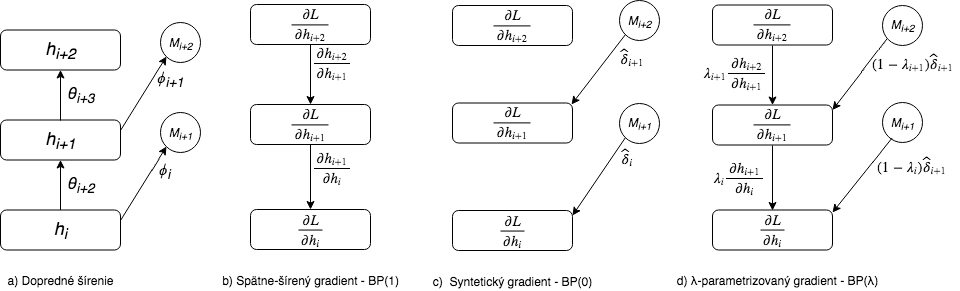
\includegraphics[width=1\textwidth]{images/BpLambda}}
%popis obrazku
\caption[Porovnanie šírenia gradientu s využitím algoritmu $BP(\lambda)$]{a) Fáza dopredného šírenia, resp. dopredná transformácia dát. Šípky opisujú, aké váhy sú použité pri jednotlivých prechodoch medzi vrstvami. b) Gradient šírený spätnou propagáciou chyby. Šípky opisujú, aká transformácia gradientu je vykonaná medzi vrstvami. c) Syntetický gradient poskytnutý modulmi syntetického gradientu. Šípky opisujú, aký syntetický gradient je poskytnutý jednotlivým vrstvám. d) Implementácia $BP(\lambda)$ algoritmu na trénovanie neurónovej siete. Výber gradientu šíreného neurónovou sieťou je podmienený parametrom $\lambda$.
\cite{Jaderberg2016}}
\label{BPlambdaAlgoritmus}
%id obrazku, pomocou ktoreho sa budeme na obrazok odvolavat
\end{figure}

V prípade algoritmu $BP(\lambda)$ nastávajú dva extrémne prípady. Berúc do úvahy, že parameter $\lambda$ stochasticky nadobúda len hodnoty 0 alebo 1, tak v parametrizovanom súčte bude výsledný $\lambda$-parametrizovaný gradient pozostávať len zo syntetického gradientu alebo len zo spätne šíreného gradientu. 

Ak $\lambda_i = 0 \quad \forall i$, tak sa jedná o štandardnú implementáciu syntetického gradientu s využitím syntetického gradientu na každej vrstve (viď Obrázok \ref{multiDNI} c)). Toto tvrdenie vyplýva z toho, že ak do definície $\lambda$-parametrizovaného gradientu $g_i$ \ref{lambdaParametrizedGradient} za parameter $\lambda$ dosadíme 0 \[    g_i=\lambda_i g_{i+1} \frac{\partial h_{i+1}}{\partial h_i}+(1-\lambda\textsubscript{i})\hat{\delta}_i=0.g_{i+1} \frac{\partial h_{i+1}}{\partial h_i}+(1-0)\hat{\delta}_i=\hat{\delta}_i\] tak zvolený gradient je vždy syntetický gradient. Druhý extrémny prípad nastáva, ak $\lambda\textsubscript{i} = 1 \quad \forall i$. V takomto prípade každá vrstva neurónovej siete využíva spätne šírený gradient. Jedná sa o model neurónovej siete, s aplikáciou štandardného spätného šírenia chyby \cite{Jaderberg2016}.

\section{Zhrnutie syntetického gradientu}
\label{SGzhrnutie}
V tejto kapitole sme objasnili trénovanie štandardnej neurónovej siete. Kľúčové bolo pochopiť spôsob šírenia gradientu sieťou za normálnych okolností vo fáze spätného šírenia chyby. Ukázali sme matematické vyjadrenie, ako sa upravujú váhy za pomoci obdržaného gradientu a ako sa tento gradient mení vzhľadom na šírenie neurónovou sieťou. Myšlienka syntetického gradientu úplne vyvrátila potrebu spätnej propagácie chyby. Implementácia modulov syntetického gradientu s ktorými komunikujú jednotlivé vrstvy neurónovej siete pomocou DNI, umožňujú týmto vrstvám upravovať svoje váhy bez závislosti na iných vrstvách. Za štandardných podmienok, vo fáze spätného šírenia chyby je vrstva $i,\quad i \in \{0,....,I-1\}$ závislá na hodnote gradientu obdržaného od vrstvy $i+1$. Výstupná vrstva $I$ obdržiava skutočný gradient, vyrátaný chybovou funkciou $L(\hat{y}, y)$ na základe chyby predikcie $\hat{y}$ a supervízie $y$. 

Trénovanie neurónovej siete pomocou spätného šírenia chyby neefektívne využíva jednotlivé zdroje, resp. vrstvy neurónovej siete \cite{Jaderberg2016}. Vrstva ktorá dokončila transformáciu dát je pripravená upraviť svoje váhy, no algoritmom spätného šírenia chyby je nútená čakať, pokiaľ všetky vrstvy pred ňou dokončia dopredné šírenie a následne upravia svoje váhy. Keďže ide o sekvenčný algoritmus ktorý má presne zadefinovaný tok krokov, tak sa nenaskytuje žiadna príležitosť na zefektívnenie prístupu k jednotlivým zdrojom neurónovej siete. 

Uvedením modulu syntetického gradientu je umožnené každej vrstve upraviť váhy ihneď po transformácii dát. Vďaka tomuto modulu syntetického gradientu, žiadna vrstva nie je nútená čakať na gradient od vyššej vrstvy.  

Zamerali sme sa na otázku, na aké typy neurónových sieti je možné aplikovať syntetický gradient. Syntetický gradient sme sa rozhodli implementovať do špeciálnej architektúry neurónovej siete zvanej reziduálna sieť. Tento typ neurónovej siete je výnimočný predovšetkým svojou hĺbkou (počtom skrytých vrstiev), ktorá sa ráta až na stovky vrstiev. Zdroj \cite{Jaderberg2016} uviedol, že implementácia syntetického gradientu je možná v akejkoľvek architektúre neurónovej siete, ktorá v rámci trénovania využíva fázu spätného šírenia chyby. 

Zdroj \cite{Jaderberg2016} a \cite{Czarnecki2017} demonštrovali fungovanie syntetického gradientu predovšetkým na rekurentných a dopredných neurónových sieťach, no svoje tvrdenie o tom, že syntetický gradient môže byť aplikovaný na akýkoľvek druh siete dokázali experimentom ktorý je opísaný v Dodatku \ref{SGexperimets} a Dodatku \ref{compareDNIandCDNI}. V tomto experimente bolo preukázané, že syntetický gradient môže byť použitý na trénovanie konvolučnej neurónovej siete ktorá na každej skrytej vrstve vykonáva lineárnu klasifikáciu realizovanú dávkovou normalizáciou a ReLU. Táto sieť v prípade použitia syntetického gradientu neprejavovala žiadne signifikantné úpadky presnosti v porovnaní s použitím gradientu šíreného spätnou propagáciou chyby.

Podobný experiment vykonal aj \cite{Czarnecki2017}, ktorý trénoval hlbokú neurónovú sieť, tiež s využitím dávkovej normalizácie a ReLU na dátovej sade MNIST \cite{yann1998mnist}. Táto neurónová sieť obsahovala vyše 50 skrytých vrstiev. Podľa vyjadrenia \cite{Czarnecki2017}, neurónová sieť s využitím syntetického gradientu dokáže lepšie konvergovať za predpokladu, že obsahuje viacej skrytých vrstiev. Zdroj \cite{Czarnecki2017} tiež uviedol, že syntetický gradient \textbf{nemal} signifikantne negatívny vplyv na presnosť tak hlbokej neurónovej siete. Na základe tohto tvrdenia sa domnievame, že syntetický gradient by mal mať podobne priaznivý dopad aj na tak hlboké neurónové siete ako sú reziduálne siete